\chapter{Organogenese: de bouw van de ledemaat van tetrapoden}\label{ch:b2:limb-organogenesis}

Drie dagen nadat een kippenei is gelegd, verschijnt aan elke flank van het
embryo een bultje zo groot als een speldenknop. Vier dagen later is het een
vleugel, met een opperarmbeen, een spaakbeen en een ellepijp, een pols en
drie vingers, in de juiste volgorde, met de juiste lengten, en met spieren
die aan de juiste botten vastzitten. Snijd de rand van verdikte huid van het
bultje weg en de vleugel houdt op met groeien; zet een reepje van de
achterrand ervan op de voorrand en er groeien zes vingers in spiegelbeeld.
De \omterm{def:b2:limb-organogenesis:bud}{ledemaatknop} is het klassieke voorbeeld van \emph{organogenese} --- de
bouw van een orgaan uit een veld van cellen door signalen die zeggen hoe ver
naar buiten, hoe ver naar voren en hoe ver naar boven elke cel ligt --- en
de experimenten die haar ontcijferden, behoren tot de helderste van de
biologie. Dit hoofdstuk volgt de knop van zijn uitgroei tot zijn skelet.

\section{De knop en zijn drie assen}

\begin{definition}[De ledemaatknop]\label{def:b2:limb-organogenesis:bud}
\index{ledemaatknop}\index{apicale ectodermale richel}\index{zone van polariserende activiteit}
De \emph{ledemaatknop} is een zwelling van \emph{mesoderm van de laterale
plaat}, bedekt met ectoderm, die ontstaat op een vaste plaats langs de
flank (het \emph{ledemaatveld}) waar de Hox-code van de lichaamsas dat
toelaat; zijn mesoderm zal bot, kraakbeen, pezen en lederhuid maken, en
cellen die er vanuit de somieten in migreren, zullen de spieren maken. De
knop heeft drie assen, elk bestuurd door een signaalcentrum.
\emph{Proximodistaal} (van schouder tot vingertop): de \emph{apicale
ectodermale richel} (AER), een verdikte strook ectoderm langs de top,
scheidt \omterm{prop:b2:limb-organogenesis:aer}{fibroblastgroeifactoren} (FGF's) af die het mesoderm eronder delend
en ongedifferentieerd houden.
\emph{Anteroposterior} (van duim tot pink): de \emph{zone van
polariserende activiteit} (ZPA), een blok mesoderm aan de achterrand,
scheidt het morfogeen \emph{\omterm{prop:b2:limb-organogenesis:zpa}{Sonic hedgehog}} (Shh) af.
\emph{Dorsoventraal} (van handrug tot handpalm): het dorsale ectoderm
scheidt Wnt7a af. Knoppen van voor- en achterpoot zien er gelijk uit en
gebruiken dezelfde signalen; ze verschillen in een transcriptiefactor die
al vóór het verschijnen van de knop tot expressie komt (Tbx5 in de
voorpoot, Tbx4 in de achterpoot), en daarom is een vleugel een vleugel.
\end{definition}

\begin{omfigure}
\begin{tikzpicture}[every node/.style={font=\scriptsize}, >=stealth]
  % flank
  \fill[omExo!25] (0,-2.2) rectangle (1.2,2.2); \node[rotate=90] at (0.6,0) {lichaamswand (flank)};
  % bud outline: paddle
  \draw[thick, fill=omDef!10] (1.2,1.4) .. controls (3.0,1.9) and (5.2,1.6) .. (5.8,0.3) .. controls (5.9,-0.3) and (5.2,-1.6) .. (3.4,-1.7) .. controls (2.4,-1.8) and (1.6,-1.5) .. (1.2,-1.4);
  % AER along the tip
  \draw[line width=3pt, omThm] (5.2,1.3) .. controls (5.9,0.6) and (5.9,-0.6) .. (5.0,-1.4);
  \node[omThm, anchor=west, align=left] at (6.1,0.9) {apicale ectodermale richel (AER):\\FGF's, proximodistale uitgroei};
  % ZPA posterior
  \draw[thick, omProp, fill=omProp!50] (2.4,-1.1) ellipse (0.55 and 0.4);
  \draw[omProp] (2.4,-1.5) -- (2.4,-2.0);
  \node[omProp, anchor=north, align=center] at (2.6,-2.0) {ZPA (achterrand):\\Sonic hedgehog, anteroposterior};
  % dorsal ectoderm
  \draw[line width=2pt, omDef!70!black] (1.4,1.55) .. controls (3.0,2.0) and (5.0,1.7) .. (5.4,1.2);
  \node[omDef!70!black, anchor=south] at (3.4,2.05) {dorsaal ectoderm: Wnt7a, dorsoventraal};
  % axes
  \draw[->, thick] (1.5,-3.1) -- (5.5,-3.1); \node[below] at (3.5,-3.15) {proximaal $\to$ distaal};
  \draw[->, thick] (10.6,-1.6) -- (10.6,1.2); \node[right, align=left] at (10.7,-0.2) {posterieur $\to$ anterieur\\(pink naar duim)};
\end{tikzpicture}

{\small De \omterm{def:b2:limb-organogenesis:bud}{ledemaatknop} van een kuiken van bovenaf gezien, met zijn drie
signaalcentra: de AER langs de top drijft de uitgroei aan, de ZPA aan de
achterrand geeft de vingers hun patroon, het dorsale ectoderm onderscheidt
rug van palm.}
\end{omfigure}

\begin{omfigure}
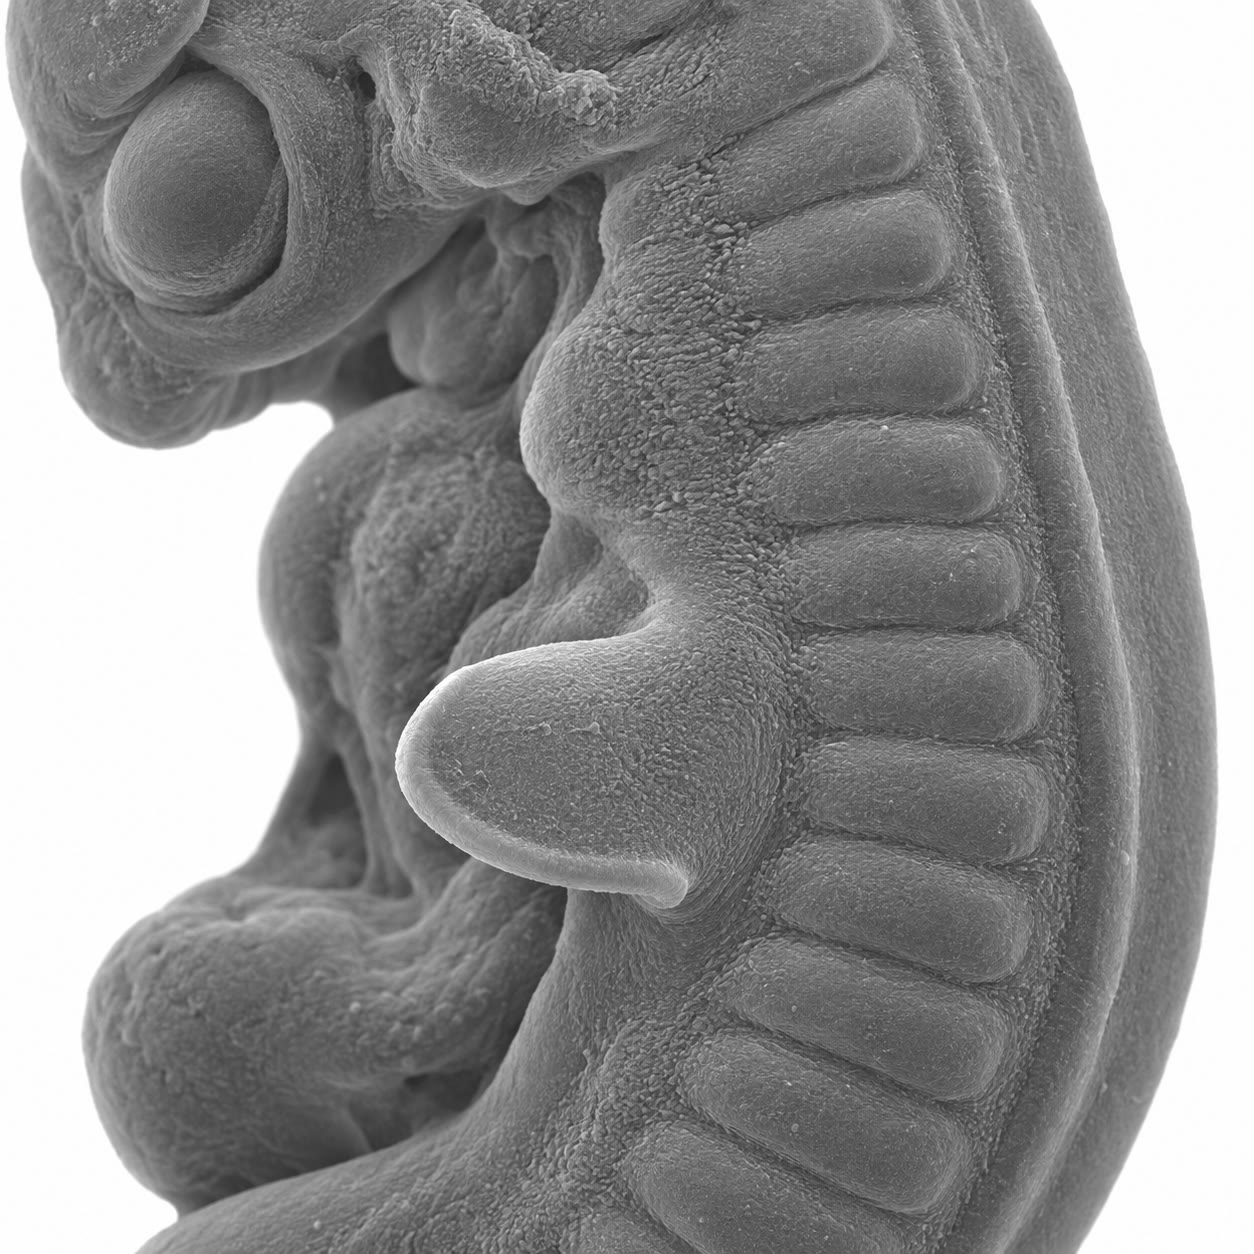
\includegraphics[width=0.42\linewidth]{images/book4/ai/b4-11-limb-bud.jpg}

{\small Een kuikenembryo onder de rasterelektronenmicroscoop: de rij
somieten langs de romp en, op de flank, de peddelvormige \omterm{def:b2:limb-organogenesis:bud}{ledemaatknop} met
de verdikte richel langs zijn rand.}
\end{omfigure}

\section{Uitgroei: de proximodistale as}

\begin{proposition}[De apicale ectodermale richel]\label{prop:b2:limb-organogenesis:aer}
\index{fibroblastgroeifactor}\index{progressiezone}
De AER is nodig voor de uitgroei en haar FGF's volstaan: het mesoderm eronder,
de \emph{\omterm{prop:b2:limb-organogenesis:aer}{progressiezone}}, deelt zich ongeveer om de twaalf uur, en cellen
die de zone verlaten naarmate de top oprukt, houden op met delen,
condenseren en differentiëren. Het skelet vormt zich in proximodistale
volgorde --- \emph{stylopodium} (opperarmbeen of dijbeen),
\emph{zeugopodium} (spaakbeen en ellepijp, scheenbeen en kuitbeen),
\emph{autopodium} (pols en vingers) --- waarbij elk segment op zijn beurt
wordt gespecificeerd terwijl de knop groeit, en de segmenten komen overeen
met geneste domeinen van Hox-genexpressie (Hoxa/d 9--10 in het stylopodium,
11 in het zeugopodium, 13 in het autopodium). Een \omterm{def:b2:limb-organogenesis:bud}{ledemaatknop} wordt in
vier dagen zo'n tien keer langer, terwijl het bereik van het signaal van de
richel dezelfde paar honderd micrometer blijft, zodat de richel de ledemaat
niet in één keer een patroon geeft maar als een oprukkend front, zoals een
printer een pagina regel voor regel neerlegt.
\end{proposition}
\begin{proof}[Bewijsmateriaal]
Saunders (1948) verwijderde de AER van vleugelknoppen van kuikens in
opeenvolgende stadia: vroeg verwijderd leverde de knop alleen een stompje
opperarmbeen op; een dag later verwijderd, opperarmbeen en onderarm maar
geen hand; nog later verwijderd, een bijna volledige vleugel --- hoe later
de ingreep, hoe distaler het niveau van de afknotting, zodat de richel
voor elk segment op zijn beurt nodig is. Het transplanteren van een tweede
richel gaf een tweede uitgroei; een kraal gedrenkt in FGF, geplaatst op een
knop waarvan de richel was verwijderd, herstelde een volledige ledemaat
(Niswander, 1993), en een kraal op de flank tussen de ledemaatvelden
induceerde een extra ledemaat. Muizen zonder de FGF's van de richel hebben
geen ledematen.
\end{proof}

\begin{omfigure}
\begin{tikzpicture}[every node/.style={font=\scriptsize}]
  \foreach \x/\lab/\n in {0/{AER vroeg verwijderd:\\alleen opperarmbeen}/1, 3.6/{een dag later verwijderd:\\opperarmbeen, spaakbeen, ellepijp}/2, 7.2/{nog later verwijderd:\\bijna volledige vleugel}/3, 10.8/{intact:\\volledige vleugel}/4} {
    \begin{scope}[xshift=\x cm]
      \fill[omExo!25] (0,-0.5) rectangle (0.5,2.6);
      % humerus
      \draw[thick, fill=omDef!25, rounded corners=3pt] (0.6,0.9) rectangle (1.7,1.2);
      \ifnum\n>1 \draw[thick, fill=omDef!25, rounded corners=3pt] (1.8,1.05) rectangle (2.7,1.3); \draw[thick, fill=omDef!25, rounded corners=3pt] (1.8,0.75) rectangle (2.7,1.0); \fi
      \ifnum\n>2 \foreach \y in {0.55,0.85,1.15} \draw[thick, fill=omDef!25, rounded corners=2pt] (2.8,\y) rectangle (3.3,\y+0.2); \fi
      \ifnum\n=4 \foreach \y in {0.55,0.85,1.15} \draw[thick, fill=omDef!25, rounded corners=2pt] (3.35,\y) rectangle (3.5,\y+0.2); \fi
      \node[below, align=center] at (1.8,-0.2) {\lab};
    \end{scope}
  }
\end{tikzpicture}

{\small Het experiment van Saunders. Hoe vroeger de richel wordt
verwijderd, hoe meer er van de ledemaat ontbreekt, altijd vanaf de top: de
richel is voor elk segment nodig zolang dat segment wordt aangelegd.}
\end{omfigure}

\begin{theorem}[Groei door deling]\label{thm:b2:limb-organogenesis:growth}
Een knop waarvan de cellen zich om de $T$ uur delen, vermenigvuldigt zijn
aantal cellen met $2^{t/T}$ in een tijd $t$; vier dagen van cycli van twaalf uur geven
$2^{8} = 256$. Als het volume van de knop in die vier dagen duizendvoudig
groeit, levert deling een factor 256 en moet de resterende factor vier
komen van celvergroting en van de matrix die kraakbeencellen om zich heen
afscheiden. Omgekeerd komt een segment waarvan de specificatie één
celcyclus vergt --- de ongeveer twaalf uur die de opeenvolgende
afknottingsniveaus van het experiment van Saunders van elkaar scheiden ---
overeen met één verdubbeling van de \omterm{prop:b2:limb-organogenesis:aer}{progressiezone}.
\end{theorem}
\begin{proof}
$N(t) = N_0 2^{t/T}$; met $t = \qty{96}{h}$ en $T = \qty{12}{h}$ is
$t/T = 8$. De verhouding van de vereiste factor tot de factor door deling,
$1000/256 \approx 4$, is wat andere groei dan deling moet leveren.
\end{proof}

\section{Vingers: de anteroposterieure as}

\begin{proposition}[De zone van polariserende activiteit]\label{prop:b2:limb-organogenesis:zpa}
\index{Sonic hedgehog}\index{morfogeen!Shh}
De ZPA bepaalt welke vinger zich waar vormt. Haar cellen scheiden \omterm{prop:b2:limb-organogenesis:zpa}{Sonic
hedgehog} af, dat zich vanaf de achterrand over de knop verspreidt, en
mesodermcellen lezen de concentratie --- en de tijd dat ze eraan zijn
blootgesteld --- als een positie: de hoogste dosis geeft de meest
posterieure vinger, lagere doses meer anterieure, en onder een drempel
helemaal geen vinger. De gradiënt heeft de exponentiële vorm van
\cref{ch:b2:vertebrate-development}, met een vervallengte van enkele
tientallen micrometers, en zijn drempels verdelen de knop in de aanleg van
de vingers: in de vleugel van een kuiken, van posterieur naar anterieur,
vinger 4, 3 en 2. Een tweede bron van het signaal aan de voorrand geeft een
tweede reeks in spiegelbeeld; een zwakkere bron, of een kortere
blootstelling, geeft alleen de anterieure vingers van de extra reeks.
Hetzelfde gen geeft, in dezelfde rol, de vingers van elke tetrapode hun
patroon, en een \omterm{def:b2:genome-diversification:mutation}{mutatie} die een anterieure bron van
Shh toevoegt, geeft polydactylie bij katten, kippen, muizen en mensen.
\end{proposition}
\begin{proof}[Bewijsmateriaal]
Saunders en Gasseling (1968) transplanteerden een blok mesoderm van de
achterrand van de ene vleugelknop naar de voorrand van een andere: de
gastheer kreeg een vleugel met zes vingers in de volgorde 4-3-2-2-3-4, een
spiegelbeeld rond het midden. Tickle (1975) toonde aan dat het aantal extra
vingers afhing van het aantal getransplanteerde cellen --- een dosis.
Riddle en Tabin (1993) vonden dat het getransplanteerde weefsel het gen
\emph{\omterm{prop:b2:limb-organogenesis:zpa}{Sonic hedgehog}} tot expressie bracht, dat het gen nergens anders in de
knop tot expressie kwam, en dat cellen die zo waren gemodificeerd dat ze het
tot expressie brachten, anterieur getransplanteerd, de verdubbeling in
spiegelbeeld reproduceerden; een kraal met het eiwit deed hetzelfde.
Kuikenmutanten met een ectopische anterieure plek van Shh hebben extra
anterieure vingers.
\end{proof}

\begin{omfigure}
\begin{tikzpicture}[every node/.style={font=\scriptsize}, >=stealth]
  % normal bud with gradient and digits
  \begin{scope}
    \fill[omExo!25] (0,-0.3) rectangle (0.4,3.3);
    \shade[bottom color=omProp!60, top color=white] (0.4,-0.3) rectangle (3.2,3.3);
    \draw[thick] (0.4,-0.3) rectangle (3.2,3.3);
    \draw[thick, omProp, fill=omProp!70] (0.9,0.1) ellipse (0.45 and 0.35); \node[omProp!80!black, anchor=west] at (1.4,0.1) {ZPA};
    \foreach \y/\d in {0.6/4, 1.5/3, 2.4/2} { \draw[thick, fill=omDef!25, rounded corners=2pt] (3.3,\y-0.12) rectangle (4.2,\y+0.12); \node[right] at (4.25,\y) {vinger \d}; }
    \node[below, align=center] at (2.0,-0.5) {normale knop: Shh vanaf de\\achterrand, vingers 4-3-2};
    \draw[->, thick] (-0.4,0.2) -- (-0.4,3.0); \node[rotate=90] at (-0.7,1.6) {posterieur $\to$ anterieur};
  \end{scope}
  % grafted bud
  \begin{scope}[xshift=7cm]
    \fill[omExo!25] (0,-0.3) rectangle (0.4,3.3);
    \shade[bottom color=omProp!60, top color=white] (0.4,-0.3) rectangle (3.2,1.5);
    \shade[top color=omProp!60, bottom color=white] (0.4,1.5) rectangle (3.2,3.3);
    \draw[thick] (0.4,-0.3) rectangle (3.2,3.3);
    \draw[thick, omProp, fill=omProp!70] (0.9,0.1) ellipse (0.45 and 0.35);
    \draw[thick, omProp, fill=omProp!70] (0.9,2.9) ellipse (0.45 and 0.35); \node[omProp!80!black, anchor=west] at (1.4,2.9) {getransplanteerde ZPA};
    \foreach \y/\d in {0.3/4, 0.8/3, 1.3/2, 1.7/2, 2.2/3, 2.7/4} { \draw[thick, fill=omDef!25, rounded corners=2pt] (3.3,\y-0.1) rectangle (4.2,\y+0.1); \node[right] at (4.25,\y) {\d}; }
    \node[below, align=center] at (2.0,-0.5) {ZPA anterieur getransplanteerd:\\verdubbeling in spiegelbeeld 4-3-2-2-3-4};
  \end{scope}
\end{tikzpicture}

{\small De polariserende zone. Links: Shh verspreidt zich vanaf de
achterrand en zijn dalende concentratie specificeert vinger 4, 3 en 2.
Rechts: een tweede ZPA, naar de voorrand getransplanteerd, maakt een tweede
gradiënt en een reeks vingers in spiegelbeeld.}
\end{omfigure}

\begin{theorem}[Vingergrenzen uit de gradiënt]\label{thm:b2:limb-organogenesis:thresholds}
Met Shh in concentratie $c_0$ aan de achterrand en een vervallengte
$\lambda$ ligt de grens van het territorium van een vinger met drempel
$T_i$ op $x_i = \lambda\ln(c_0/T_i)$ van de rand. Met
$\lambda = \qty{50}{\micro m}$ en drempels van $0.6$,
$0.25$ en $0.08$ van $c_0$ voor vinger 4, 3 en 2 zijn de territoria
$0$--$26$, $26$--$69$ en $69$--$126$ micrometer, en vormt het weefsel
voorbij \qty{126}{\micro m} geen vinger. Verdubbeling van de bron
verschuift elke grens naar buiten met $\lambda\ln 2 = \qty{35}{\micro m}$
--- genoeg, in een knop van enkele honderden micrometers, om aan de
anterieure rand een vinger toe te voegen; een tweede bron aan de voorrand
legt dezelfde territoria in omgekeerde volgorde aan.
\end{theorem}
\begin{proof}
Uit $c(x) = c_0 e^{-x/\lambda}$ volgt $c = T_i$ bij $x_i = \lambda
\ln(c_0/T_i)$: $50\ln(1/0.6) = 25.5$, $50\ln 4 = 69$, $50\ln 12.5 =
126$. Vervangen van $c_0$ door $2c_0$ telt $\lambda\ln 2$ bij elke $x_i$ op.
\end{proof}

\begin{omfigure}
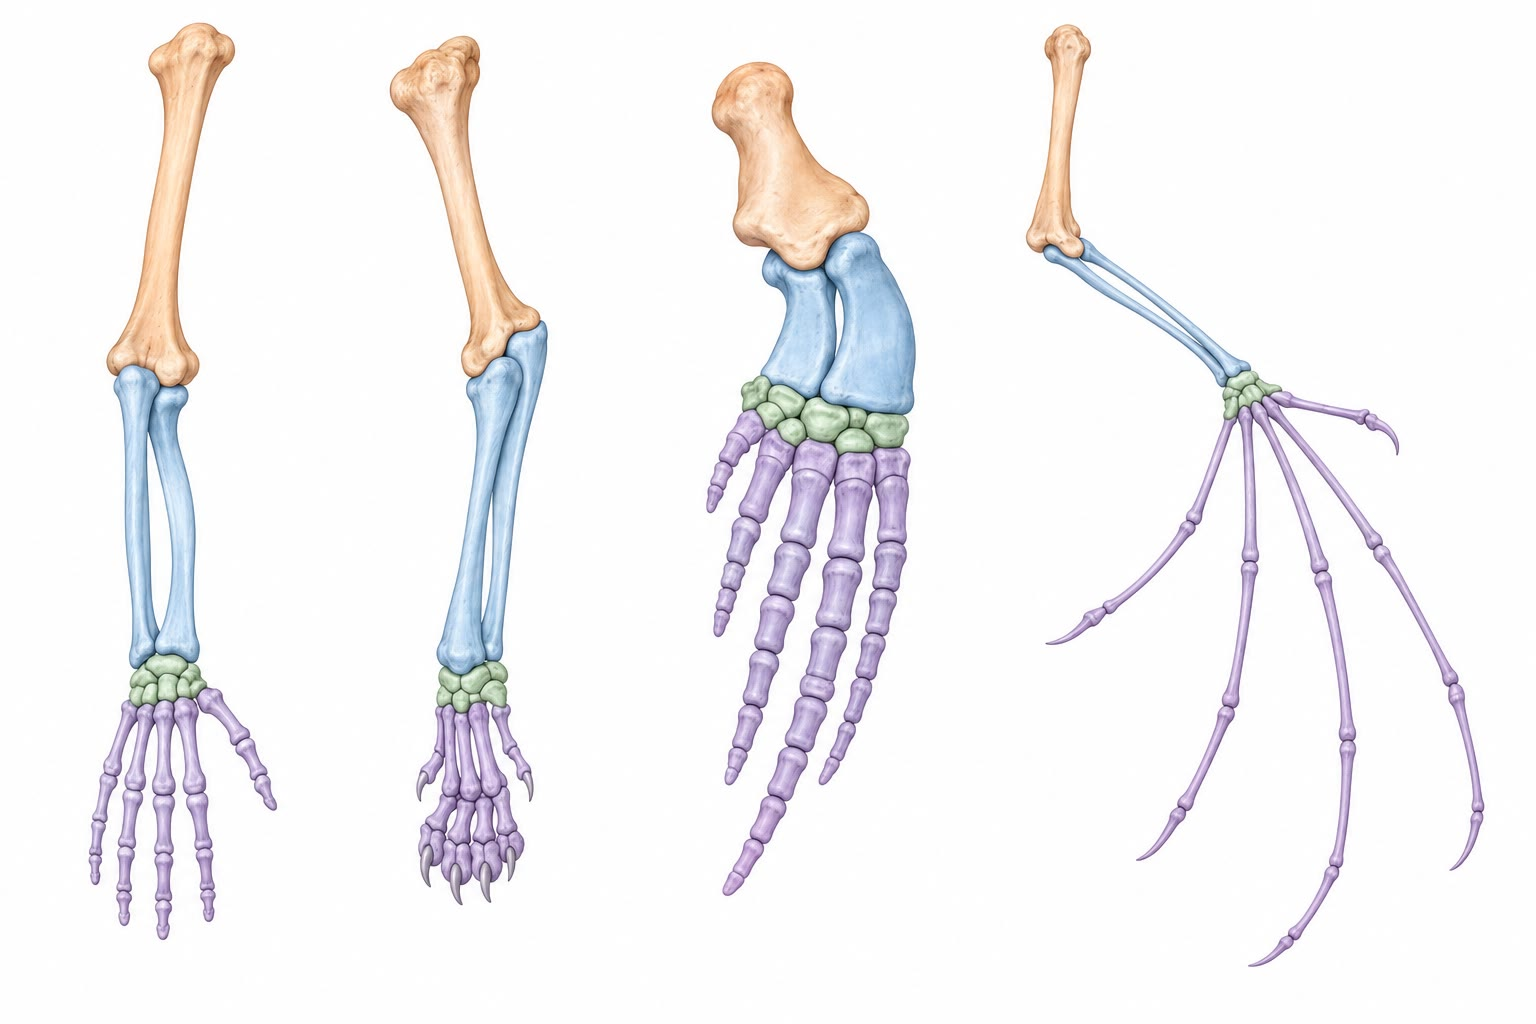
\includegraphics[width=0.66\linewidth]{images/book4/ai/b4-11-tetrapod-limbs.jpg}

{\small Eén plan, vier ledematen: de voorpoten van een mens, een kat, een
walvis en een vleermuis delen dezelfde botten in dezelfde volgorde --- één
stylopodium, twee zeugopodiumbotten, pols, vingers ---, gebouwd door
dezelfde signaalcentra en verschillend in groei.}
\end{omfigure}

\section{Coördinatie en beeldhouwen}

\begin{proposition}[De assen praten met elkaar]\label{prop:b2:limb-organogenesis:loop}
\index{terugkoppelingslus!in de ontwikkeling}
De centra houden elkaar in stand: FGF uit de richel laat de ZPA Shh tot
expressie brengen, en Shh laat, via een doorgeefluik in het mesoderm, de
richel FGF tot expressie brengen; verwijder een van beide en de ander dooft
binnen een dag uit. Wnt7a uit het dorsale ectoderm is eveneens nodig voor
volledige expressie van Shh, en het stuurt het dorsale lot van het
mesoderm aan (een muis zonder Wnt7a heeft twee handpalmen). Deze wederzijdse
afhankelijkheid is een \emph{positieve terugkoppelingslus} die de drie
assen aan elkaar koppelt: de ledemaat groeit alleen waar hij een patroon
krijgt, en krijgt alleen een patroon waar hij groeit, zodat een knop nooit
een hand zonder arm maakt of vingers van de verkeerde soort. Wanneer de
uitgroei voltooid is, wordt de lus verbroken --- het mesoderm geeft niets
meer door, Shh stopt, de richel gaat in regressie --- en houdt de ledemaat
op zijn juiste grootte op met groeien.
\end{proposition}

\begin{proposition}[Van patroon tot bot]\label{prop:b2:limb-organogenesis:skeleton}
\index{chondrogenese}\index{apoptose!interdigitale}
Eenmaal gespecificeerd \emph{condenseren} mesodermcellen die de
\omterm{prop:b2:limb-organogenesis:aer}{progressiezone} verlaten tot staven en platen met de vorm van de toekomstige
botten, differentiëren ze tot kraakbeencellen die een matrix rijk aan
collageen en proteoglycanen afscheiden, en leggen ze van elk
skeletelement een kraakbeenmodel aan; gewrichten ontstaan waar een band
cellen te horen krijgt geen kraakbeen te worden; bloedvaten dringen de
modellen binnen en bot vervangt kraakbeen van het midden naar buiten,
waarbij aan de uiteinden groeischijven overblijven die het bot tot de
volwassenheid laten verlengen (\emph{endochondrale ossificatie}).
Spiervoorlopers uit de somieten migreren binnen, delen zich, versmelten
tot vezels (\cref{ch:b2:cell-differentiation}) en hechten zich via pezen
die door het eigen mesoderm van de ledemaat worden gemaakt. Tussen de
vingerstralen wordt het weefsel door geprogrammeerde celdood verwijderd: de
cellen van de interdigitale vliezen activeren, op een signaal van een
botmorfogenetisch eiwit (BMP), hun eigen vernietiging en worden binnen een
dag opgeruimd, wat de vingers van elkaar scheidt. Een eend behoudt zijn
zwemvliezen omdat in zijn interdigitale weefsel een BMP-remmer tot
expressie komt; een kuiken dat dezelfde remmer op een kraal krijgt, krijgt
zwemvliezen.
\end{proposition}
\begin{proof}[Bewijsmateriaal]
Interdigitaal mesoderm dat uit een beenknop van een kuiken wordt gesneden
en elders wordt getransplanteerd, sterft volgens schema --- de dood is
intrinsiek en werd al beslist voordat het weefsel werd verwijderd;
hetzelfde weefsel van een eend overleeft. Kralen met BMP tussen de tenen van
een eend laten het zwemvlies afsterven; kralen met de remmer gremlin tussen
de tenen van een kuiken redden het. Een muis zonder BMP-receptor in de
ledemaat behoudt zijn vliezen.
\end{proof}

\begin{omfigure}
\begin{tikzpicture}[every node/.style={font=\scriptsize}]
  \foreach \x/\lab in {0/{vingerstralen condenseren\\als kraakbeen}, 4.2/{interdigitale cellen\\sterven (BMP)}, 8.4/{vingers gescheiden;\\bot vervangt kraakbeen}} {
    \begin{scope}[xshift=\x cm]
      \node[below, align=center] at (1.5,-0.3) {\lab};
    \end{scope}
  }
  % stage 1: paddle with rays
  \draw[thick, fill=omDef!8] (0,0) .. controls (0,2.2) and (3,2.2) .. (3,0) -- cycle;
  \foreach \x in {0.6,1.2,1.8,2.4} \draw[thick, fill=omDef!30, rounded corners=2pt] (\x-0.12,0.1) rectangle (\x+0.12,1.5);
  % stage 2: paddle with dying webs
  \begin{scope}[xshift=4.2cm]
    \draw[thick, fill=omDef!8] (0,0) .. controls (0,2.2) and (3,2.2) .. (3,0) -- cycle;
    \foreach \x in {0.6,1.2,1.8,2.4} \draw[thick, fill=omDef!30, rounded corners=2pt] (\x-0.12,0.1) rectangle (\x+0.12,1.5);
    \foreach \x in {0.9,1.5,2.1} \foreach \y in {0.7,1.0,1.3} \fill[omThm] (\x,\y) circle (0.05);
  \end{scope}
  % stage 3: separated digits
  \begin{scope}[xshift=8.4cm]
    \draw[thick, fill=omDef!8] (0,0) -- (0,0.5) -- (0.3,0.5) -- (0.35,1.7) -- (0.85,1.7) -- (0.9,0.5) -- (1.05,0.5) -- (1.1,1.85) -- (1.6,1.85) -- (1.65,0.5) -- (1.8,0.5) -- (1.85,1.7) -- (2.35,1.7) -- (2.4,0.5) -- (2.7,0.5) -- (2.7,0) -- cycle;
    \foreach \x in {0.6,1.35,2.1} \draw[thick, fill=omExo!60, rounded corners=2pt] (\x-0.1,0.1) rectangle (\x+0.1,1.4);
  \end{scope}
\end{tikzpicture}

{\small Het beeldhouwen van de hand: kraakbeenstralen condenseren in de
peddel, de cellen ertussen sterven (rood), en de vrijgekomen vingers verbenen.}
\end{omfigure}

\begin{example}[Dezelfde ledemaat, anders gegroeid]\label{ex:b2:limb-organogenesis:evolution}
De vleugel van een vleermuis is een hand waarvan de vingers 2 tot 5
meermaals langer uitgroeiden dan die van een muis --- een enhancer van een
ledemaatgen, van vleermuis naar muis overgebracht, verlengt de botten van de
voorpoot van de muis --- en waarvan het interdigitale weefsel overleefde,
omdat het vlies de BMP-remmer tot expressie brengt die ook de eend
gebruikt. De flipper van een walvis is een hand met extra kootjes en zonder
interdigitale celdood. Het been van een paard is één enkele vinger, met de
andere teruggebracht tot griffelbeentjes. De slang heeft geen ledematen omdat
haar flank de signalen die een knop starten nooit tot expressie brengt. En
de vinnen van vissen, die geen autopodium hebben, worden gebouwd door
dezelfde AER en ZPA, maar breken hun Hox-programma af vóór de late fase die
vingers maakt; het fossiel \emph{Tiktaalik} (375 miljoen jaar oud) laat de
pols in een vin zien verschijnen. De evolutie van ledematen is vooral de
modulatie van een geconserveerd programma --- hoe lang elke fase duurt, hoe
ver elk signaal reikt, welke cellen sterven.
\end{example}

\section{Opgaven}

\begin{exercise}[$\star$]\label{exo:b2:limb-organogenesis:1}
Noem de drie assen van de \omterm{def:b2:limb-organogenesis:bud}{ledemaatknop} en, voor elk, het signaalcentrum, zijn
positie en zijn signaal.
\end{exercise}

\begin{exercise}[$\star$]\label{exo:b2:limb-organogenesis:2}
Geef de drie segmenten van het skelet van de ledemaat en de botten van elk
in een menselijke arm en een menselijk been. Welke Hox-genen markeren ze?
\end{exercise}

\begin{exercise}[$\star$]\label{exo:b2:limb-organogenesis:3}
Noem in volgorde de stappen van een stukje mesoderm van de laterale plaat
tot een vinger met zijn bot, gewricht en spier.
\end{exercise}

\begin{exercise}[$\star$]\label{exo:b2:limb-organogenesis:4}
Hoe ziet de ledemaat eruit als de AER wordt verwijderd (a) zodra de knop
verschijnt, (b) nadat de onderarm is gespecificeerd, (c) helemaal niet,
maar vervangen door een kraal met FGF?
\end{exercise}

\begin{exercise}[$\star\star$]\label{exo:b2:limb-organogenesis:5}
Bereken met $\lambda = \qty{40}{\micro m}$ en drempels van $0.5$, $0.2$
en $0.05$ van de bronconcentratie voor vinger 4, 3 en 2 de drie grenzen en
de breedte van elk vingerterritorium.
\end{exercise}

\begin{exercise}[$\star\star$]\label{exo:b2:limb-organogenesis:6}
Voorspel het vingerpatroon van een vleugel van een kuiken na (a) een
volledige ZPA die naar de voorrand wordt getransplanteerd, (b) een
transplantaat van een kwart zoveel ZPA-cellen, (c) een kraal met Shh aan de
voorrand die na een korte blootstelling wordt verwijderd. Verklaar elk
geval met dosis en tijd.
\end{exercise}

\begin{exercise}[$\star\star$]\label{exo:b2:limb-organogenesis:7}
Een \omterm{def:b2:limb-organogenesis:bud}{ledemaatknop} van een kuiken telt \num{5000} cellen wanneer de richel zich
vormt, en zijn cellen delen zich om de \qty{12}{h}. Hoeveel cellen zijn er
na vier dagen? Als de ledemaat in dat stadium $4\times 10^{6}$ cellen telt,
wat moet er dan gelden voor de celcyclus of voor celdood?
\end{exercise}

\begin{exercise}[$\star\star$]\label{exo:b2:limb-organogenesis:8}
Leg uit waarom een kuiken vrije tenen heeft en een eend zwemvliezen, en wat
een kraal met BMP-remmer tussen de tenen van een kuikenembryo doet. Wat zegt
de intrinsieke timing van de interdigitale celdood (ze treedt in een
transplantaat volgens schema op) over de manier waarop de cellen werden
geïnstrueerd?
\end{exercise}

\begin{exercise}[$\star\star$]\label{exo:b2:limb-organogenesis:9}
Een muis mist zowel Hoxa13 als Hoxd13; een andere mist Hoxa11 en
Hoxd11. Voorspel het skelet van elke voorpoot en zeg wat het resultaat
aantoont over de relatie tussen Hox-domeinen en segmenten.
\end{exercise}

\begin{exercise}[$\star\star\star$]\label{exo:b2:limb-organogenesis:10}
Leg de positieve terugkoppeling tussen de AER en de ZPA uit, waarom ze de
ledemaat robuust maakt, en wat er zou gebeuren met een knop waarin Shh FGF
niet in stand kon houden. Vergelijk met de positieve terugkoppeling van de
bevalling in \cref{ch:b2:mammal-reproduction}: wat beëindigt elke lus?
\end{exercise}

\begin{exercise}[$\star\star\star$]\label{exo:b2:limb-organogenesis:11}
De derde vinger van een vleermuis is, relatief ten opzichte van de
lichaamsgrootte, acht keer langer dan die van een muis. Als het kraakbeen
van een vinger tijdens een groeivenster exponentieel verlengt met snelheid
$r$ per dag, en het venster van de vleermuis vier dagen langer duurt dan
dat van de muis, welke $r$ is dan nodig? Geef twee
ontwikkelingsveranderingen (één in groei, één in celdood) die van een hand
een vleugel maken.
\end{exercise}

\begin{exercise}[$\star\star\star$]\label{exo:b2:limb-organogenesis:12}
\omterm{prop:b2:limb-organogenesis:zpa}{Sonic hedgehog} geeft de \omterm{prop:b2:vertebrate-development:neurulation}{neurale buis} een patroon vanuit de bodemplaat
(\cref{ch:b2:vertebrate-development}) en de vingers vanuit de ZPA.
Bespreek waarom de evolutie een paar signalen voor veel taken hergebruikt,
hoe hetzelfde molecuul in verschillende weefsels verschillende dingen kan
betekenen, en wat dit inhoudt voor het effect van een \omterm{def:b2:genome-diversification:mutation}{mutatie} in zo'n gen.
\end{exercise}

\section{Vraagstuk: een vleugel gebouwd in een week}

\begin{problem}[{Weekendvraagstuk --- de vleugel van een kuiken gevolgd van
knop tot skelet: zijn groei door deling, de richelverwijderingen van
Saunders getimed, de Shh-gradiënt berekend en zijn verdubbelingen voorspeld,
de vliezen weggebeeldhouwd en de vleugel vergeleken met die van een
vleermuis, met als besluit het aantal verdubbelingen, de vingergrenzen en de
breedte die een knop nodig heeft voor een verdubbeling in spiegelbeeld}]
\label{pb:b2:limb-organogenesis:1}
Een vleugelknop van een kuiken verschijnt na 3 dagen broeden met \num{2000}
mesodermcellen en een lengte van \qty{0.4}{mm}; na 7 dagen is de vleugel
\qty{4}{mm} lang en is zijn volume \num{1000} keer dat van de knop. Cellen
van de \omterm{prop:b2:limb-organogenesis:aer}{progressiezone} delen zich om de \qty{12}{h}. Richelverwijderingen:
bij 3.0 dagen is de ledemaat een stompje; bij 3.5 dagen alleen een
opperarmbeen; bij 4.0 dagen opperarmbeen, spaakbeen en ellepijp; bij 4.5
dagen een vleugel waaraan alleen de vingertoppen ontbreken.
Shh: $D = \qty{1e-12}{m^2/s}$, halveringstijd \qty{29}{min}; drempels
$0.6$, $0.25$, $0.08$ van $c_0$ voor vinger 4, 3, 2. Breedte van de knop
(van posterieur naar anterieur) \qty{600}{\micro m}. Interdigitale vliezen:
drie gebieden van
\qty{300}{\micro m}$\times$\qty{300}{\micro m}$\times$\qty{200}{\micro m},
cellen van \qty{1000}{\micro m^3}, opgeruimd in \qty{24}{h}.

\medskip
\noindent\textbf{Deel I --- Groei.}
\begin{enumerate}
  \item Hoeveel verdubbelingen vinden er in vier dagen plaats? Hoeveel
        cellen levert dat op vanaf \num{2000}?
  \item Vergelijk met de duizendvoudige volumetoename: welke factor moeten
        celvergroting en matrix leveren?
  \item Met welke factor groeide de lengte? Als de knop groeide als een
        cilinder met constante straal, welke volumefactor zou dat zijn, en
        wat zegt het verschil over de vorm?
  \item Het FGF van de richel reikt \qty{300}{\micro m} ver het mesoderm in.
        Welk deel van de knop staat na 3 dagen en na 7 dagen onder zijn
        invloed?
  \item Leg uit waarom een signaal met een vast bereik in een groeiend
        orgaan een proximodistale opeenvolging voortbrengt.
  \item Een cel verlaat de \omterm{prop:b2:limb-organogenesis:aer}{progressiezone} na 4 dagen. Bij welk segment
        sluit ze aan?
\end{enumerate}

\medskip
\noindent\textbf{Deel II --- De segmenten getimed.}
\begin{enumerate}[resume]
  \item Geef uit de reeks verwijderingen het tijdstip waarop elk segment
        (stylopodium, zeugopodium, autopodium) is gespecificeerd.
  \item Hoeveel celcycli scheiden de specificatie van opeenvolgende
        segmenten?
  \item Verklaar het resultaat in termen van de \omterm{prop:b2:limb-organogenesis:aer}{progressiezone} en de
        Hox-domeinen.
  \item Op een knop waarvan de richel na 3.5 dagen is verwijderd, wordt een
        kraal met FGF geplaatst. Voorspel de ledemaat.
  \item Na 3.5 dagen wordt een tweede richel op het dorsale oppervlak van
        een intacte knop getransplanteerd. Voorspel.
  \item Waarom houdt de knop na 7 dagen op met groeien in plaats van
        onbeperkt door te gaan?
\end{enumerate}

\medskip
\noindent\textbf{Deel III --- De gradiënt.}
\begin{enumerate}[resume]
  \item Bereken $k$ en $\lambda$ voor Shh.
  \item Bereken de drie vingergrenzen en de breedte van de territoria.
  \item Hoe breed is het anterieure gebied dat in een knop van
        \qty{600}{\micro m} geen vinger vormt?
  \item Een \omterm{def:b2:genome-diversification:mutation}{mutatie} verdubbelt de productie van Shh. Bereken de grenzen
        opnieuw en zeg of er een extra vinger ontstaat, en welke.
  \item Een ZPA wordt naar de voorrand getransplanteerd. Welke minimale
        breedte van de knop laat een volledige spiegelreeks 4-3-2-2-3-4 toe
        zonder overlap van de twee territoria van vinger 2? Is de knop van
        het kuiken breed genoeg?
  \item Voorspel het patroon als de knop maar \qty{200}{\micro m}
        breed was.
  \item Waarom geeft een transplantaat van een kwart van de ZPA alleen 2-2-3-4?
\end{enumerate}

\medskip
\noindent\textbf{Deel IV --- Beeldhouwen en evolutie.}
\begin{enumerate}[resume]
  \item Bereken het aantal cellen in de drie vliezen en het tempo van de
        celdood tijdens het opruimen, in cellen per seconde.
  \item De interdigitale cellen van een eend brengen een BMP-remmer tot
        expressie. Voorspel het effect van een kraal met BMP in een
        eendenvlies en van de remmer in een kuikenvlies.
  \item Het vingerkraakbeen van een vleermuis groeit vier extra dagen met
        een exponentiële snelheid van \qty{0.5}{d^{-1}}. Met welke factor is
        het langer dan dat van het kuiken? Noem een tweede verandering die
        het vleugelmembraan maakt.
  \item Een vinknop van een vis heeft een AER en een ZPA, maar geen vingers.
        Wat ontbreekt er, en wat laat \emph{Tiktaalik} zien?
  \item Als de vliescellen in plaats daarvan door deling uit \num{1000}
        stichtercellen waren gemaakt, bij \qty{12}{h} per cyclus, hoelang
        zou het maken ervan dan hebben geduurd? Vergelijk met de dag die het
        verwijderen kost.
  \item Formuleer het resultaat: het aantal verdubbelingen in vier dagen,
        de drie vingergrenzen, en de minimale breedte voor een verdubbeling
        in spiegelbeeld.
\end{enumerate}
\end{problem}
